\medskip

\begin{enumerate}
\item Affirmation 1 : Vraie

Pour tout entier naturel $n$ : $n\geqslant 0 \Longrightarrow n+1 \geqslant 1 \Longrightarrow \dfrac{1}{n+1} \leqslant 1$  et  $-\dfrac{1}{n+1} \geqslant -1$.

De plus,  pour tout entier naturel $n$, $-1 \leqslant (-1)^n \leqslant 1 $.

D'où $ \dfrac{-1}{n+1} \leqslant \dfrac{(-1)^n}{n+1} \leqslant \dfrac{1}{n+1}$ car $n+1 >0$

finalement on a : $-1 \leqslant \dfrac{-1}{n+1} \leqslant \dfrac{(-1)^n}{n+1} \leqslant \dfrac{1}{n+1}\leqslant 1$.

La suite $u$ est bornée par -1 et 1.

\item Affirmation 2 : Fausse

Pour montrer qu'une affirmation est fausse, il suffit de donner un contre-exemple :

Considérons la suite $u$ définie sur $\N$ par $u_n= (-1)^n$.

Cette suite est bornée par $-1$ et 1 mais elle n'est pas convergente.

\item Affirmation 3 : Fausse

Pour montrer qu'une affirmation est fausse, il suffit de donner un contre-exemple :

Considérons la suite $u$ définie sur $\N$ par $u_n=-\dfrac{1}{n}$.

Cette suite est croissante et converge vers 0.

\item Affirmation 4 : Fausse 

Pour étudier la convexité d'une fonction,  il faut déterminer le signe de sa dérivée seconde. 

$f$ est dérivable sur $\R$ comme composée de fonctions dérivables.

$f$ est de la forme $\ln(u)$ avec $u(x)=x^2+2x+2$.  On a $u'(x)=2x+2$.

$f'=\dfrac{u'}{u}$ donc, pour tout réel $x$, $f'(x)=\dfrac{2x+2}{x^2+2x+2}$.

$f'$ est de la forme $\dfrac{v}{w}$ avec $v(x)=2x+2$ et $w(x)=x^2+2x+2$.

On a $v'(x)=2$ et $w'(x)=2x+2$.

$f''= \dfrac{v'\times w - w'\times v}{w^2}$  donc,  pour tout réel $x$,  $f''(x) =\dfrac { 2\times (x^2+2x+2)- (2x+2)\times(2x+2)    }{ {\left( x^2+2x+2 \right)}^2}$ 

$f''(x)=\dfrac {  2x^2+4x+4-4x^2-8x-4  }{ {\left( x^2+2x+2 \right)}^2} =\dfrac {  -2x^2-4x  }{ {\left( x^2+2x+2 \right)}^2} =\dfrac{-2x(x+2)}{ {\left( x^2+2x+2 \right)}^2}$.

Un carré est toujours strictement positif, $f''(x)$ est donc du signe de $-2x(x+2)$ qui est une fonction polynôme du second degré avec un coefficient dominant négatif (-2) et qui a pour racines 0 et -2.

On a donc le tableau de signe suivant :


\begin{center}
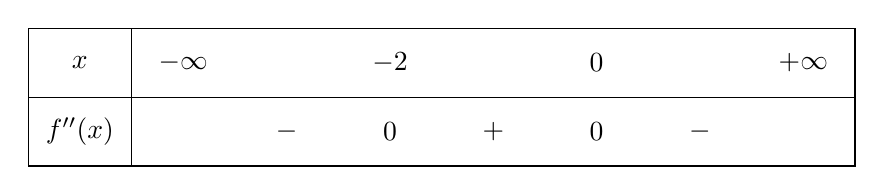
\begin{tikzpicture}[scale=0.875]

\tikzstyle{cadre}=[thin]
\tikzstyle{fleche}=[->,>=latex,thin]
\tikzstyle{nondefini}=[lightgray]

\def\Lrg{1.5}
\def\HtX{1}
\def\HtY{0.5}

\def\lignex{-0.5*\HtX}
\def\lignef{-1.5*\HtX}
\def\separateur{-0.5*\Lrg}

\def\gauche{-1.5*\Lrg}
\def\droite{6.5*\Lrg}

\def\haut{0.5*\HtX}
\def\bas{-2.5*\HtX-2*\HtY}

\node at (-1*\Lrg,0) {$x$};
\node at (0*\Lrg,0) {$-\infty$};
\node at (2*\Lrg,0) {$-2$};
\node at (4*\Lrg,0) {$0 $};
\node at (6*\Lrg,0) {$+\infty$};

\node at (-1*\Lrg,-1*\HtX) {$f''(x)$};
\node at (0*\Lrg,-1*\HtX) {$$};
\node at (1*\Lrg,-1*\HtX) {$-$};
\node at (2*\Lrg,-1*\HtX) {$0$};
\node at (3*\Lrg,-1*\HtX) {$+$};
\node at (4*\Lrg,-1*\HtX) {$0$};
\node at (5*\Lrg,-1*\HtX) {$-$};
\node at (6*\Lrg,-1*\HtX) {$$};


\draw[cadre] (\separateur,\haut) -- (\separateur, \lignef);
\draw[cadre] (\gauche,\haut) rectangle  (\droite, \lignef);
\draw[cadre] (\gauche,\lignex) -- (\droite,\lignex);
\end{tikzpicture}
\end{center}











On a déduit que $f$ est concave sur $]-\infty~;~-2]$ et sur $[0~;~+\infty[$,  et elle est convexe sur $[-2~;~0]$.

Elle n'est donc pas convexe sur $[-3~;~1]$.

\item  Affirmation 5 :  vraie

On initialise $M$ avec le premier terme de la suite, puis l'algorithme  va comparer chaque terme de la liste à $M$,  si un terme est supérieur à $M$, il va remplacer $M$.

Cet algorithme donne donc la valeur maximale des termes de la suite, soit 7 dans notre cas.
\end{enumerate}
